\documentclass{article}
\usepackage[left=1in, right=1in, top=1in, bottom=1in]{geometry}
\usepackage[utf8]{inputenc}
\usepackage{graphicx}
\setlength{\parindent}{0pt}
\usepackage{appendix}
\usepackage{enumitem}
\usepackage{amsmath}
\usepackage{xcolor}
\usepackage{soul}
\usepackage{hyperref}
\hypersetup{
    colorlinks=true,
    linkcolor=blue,
    filecolor=magenta,      
    urlcolor=cyan,
}
 
\urlstyle{same}

\begin{document}
\begin{center}
    \Huge{Project 3 Tech Memo: \\ Color Sensor \\~\\}
    \LARGE{  May 3rd, 2019. \\~\\ Team \#17 \\ Los Ingenieros \\~\\ José Luis Gómez \\ Hammad Imam \\ Thihan Moe Kyaw \\ Daniel Spathies \\~\\ ME 250 Section \#2 \\ Professor Szwalek}
\thispagestyle{empty}
\end{center}

\newpage

\section*{Executive Summary}

\newpage
\tableofcontents

\newpage
\section{Introduction}

\newpage
\section{Problem Definition}

\newpage
\section{Functional Analysis}

\newpage
\section{Concept Generation}
\subsection{Introduction}
This section’s purpose is to present the procedure that was taken to select the concept design for the color sorting device. In this section, a morphological chart is used to generate all the possible design concepts by listing all the functions and their corresponding means. From this the top twenty or so concepts are chosen through an analysis on their practicality and ability to satisfy objectives. These concepts are listed in this section. From this a list of the top five concepts are chosen through more rigorous application of the same analysis as beforehand, these top five are also listed and justified. Finally, through the use of comparison charts the top concept is selected for manufacturing the device. 

\subsection{Definitions}
Morphological chart: A matrix in which the leftmost column is a list of all of the principal functions that our design must perform and also some of the key features it must have. \\
Design space: An imaginary intellectual region of design alternatives that contains all of the possible solutions to the design problems [1].

\subsection{Morphological Chart}
The leftmost column of the chart shows the functions that should be included in the design. To the right of the functions are the all different types of means that were found which could perform the functions. The purpose of this chart, Figure 4.3.1 is to aid in expanding the design space.

\begin{center}
    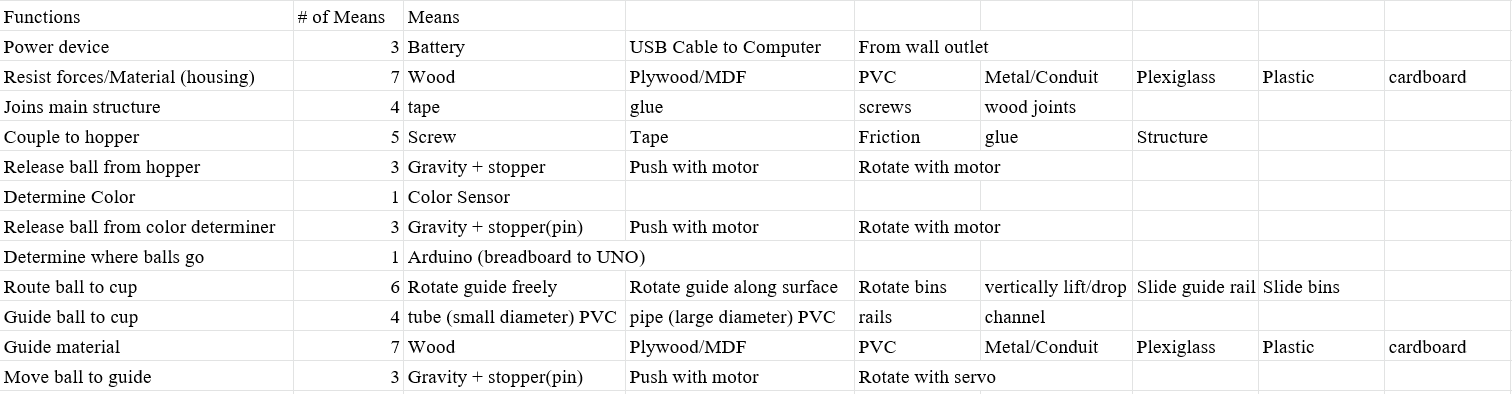
\includegraphics[width=\textwidth]{morphchart.png}\\
    \small{\textbf{Table 4.3.1} - Morphological Chart}
\end{center}

\subsection{Concept List}

\begin{itemize}
    \item   Wood housing using screws as main joiner, the color sorter is under the hopper, the ball then drops on an arm attached to a servo. The servo then rotates the calculated amount to one of the three fixed pvc pipes that lead to a cup.
    \item Cardboard housing using duct tape as main joiner, after color is sensed, a cardboard     channel is moved by a servo to align with the proper cup and then the ball is released from the color determining area and then goes down the channel into the correct cup
    \item Wood housing with screws as main joiner, also there are fixed ramps made of cardboard, the ball moves from hopper to color sensor, then the ball gets released and gets deviated dependant on arduino code to go down a different ramp which will lead to a corresponding cup 
    \item PVC housing with glue and tape as main joiners, this device acts as an elevator or dumbwaiter, after determining the color at the top of the shaft, this device drops the ball a determined height into the right cup, a servo with string can be used to lower or raise elevator shaft to desired position.
    \item Wooden housing with plastic, a spring and glue or tape as joiners, this device brings a ball from the hopper to the color sensor then drops it into a waiting catapult arm with a spring attached. The arm is pulled back at the precise distance to allow the ball to fly as a projectile and land in the correct cup, the arm is then winched back with a motor to an arduino determined distance and repeated.
    \item Wooden housing, a type of manufactured belt, metal to make conveyor and cardboard with various joiners being required. First, a single ball is deposited from the hopper and dropped onto a rotating conveyor belt that moves the ball to the right, the ball passes under the color sensor and the color is determined and then the arduino and code process the color and move a moveable ramp/platform at the end of the conveyor to bounce the ball into the correct cup.
    \item Wooden housing, a type of manufactured belt, metal to make conveyor and cardboard with various joiners being required. Similar to the other device using a conveyor, this device releases a ball onto the moving conveyor belt, scans the color and continues down the conveyor but next one of three motors is turned on and when it senses motion, extends to push to ball off the side of the conveyor into the correct cup.
    \item Wooden housing with screws or tape as main joiner, after scanning the color of the ball in the color scanning portion of the device, the ball is then dropped onto a ramp with a very small slope or angle and as the ball slowly travels down the ramp, the servo corresponding to the correct cup then moves and opens a hole for the ball to fall through into the cup below it
    \item Wooden housing with screws as main joiner, after ball’s color is sensed, the ball drops onto an arm attached to a servo, the arm rotates to be over the correct cup and then the servo on the arm activates, opening a hole in the arm, releasing the ball into the correct cup
    \item   Cardboard housing with glue and tape and main joiners, the ball gets released from hopper, color gets sensed and then after being released from the color sensing station, the ball is redirected by a servo with an extended arm to push the ball down of of the three separate paths of the connected ramp into the desired cup
\end{itemize}

\begin{center}
    Top 5 Concepts
\end{center}



\begin{itemize}
    \item Tri-Tube -  Wood housing using screws as main joiner, the color sorter is under the hopper, the ball then drops on an arm attached to a servo. The servo then rotates the calculated amount to one of the three fixed pvc pipes that lead to a cup.
    \item Moving channel -   Cardboard housing using duct tape as main joiner, after color is sensed, a cardboard channel is moved by a servo to align with the proper cup and then the ball is released from the color determining area and then goes down the channel into the correct cup
    \item Conveyor belt -  Wooden housing, a type of manufactured belt, metal to make conveyor and cardboard with various joiners being required. First, a single ball is deposited from the hopper and dropped onto a rotating conveyor belt that moves the ball to the right, the ball passes under the color sensor and the color is determined and then the arduino and code process the color and one of three motors pushes the ball when motion is sensed into the correct cup
    \item  Arm controller - Wooden housing with screws as main joiner, after ball’s color is sensed, the ball drops onto an arm attached to a servo, the arm rotates to be over the correct cup and then the servo on the arm activates, opening a hole in the arm, releasing the ball into the correct cup
    \item Tri-fold ramp- Cardboard housing with glue and tape and main joiners, the ball gets released from hopper, color gets sensed and then after being released from the color sensing station, the ball is redirected by a servo with an extended arm to push the ball down of of the three separate paths of the connected ramp into the desired cup
\end{itemize}

\subsection{Top 5 Drawings}

\begin{center}
    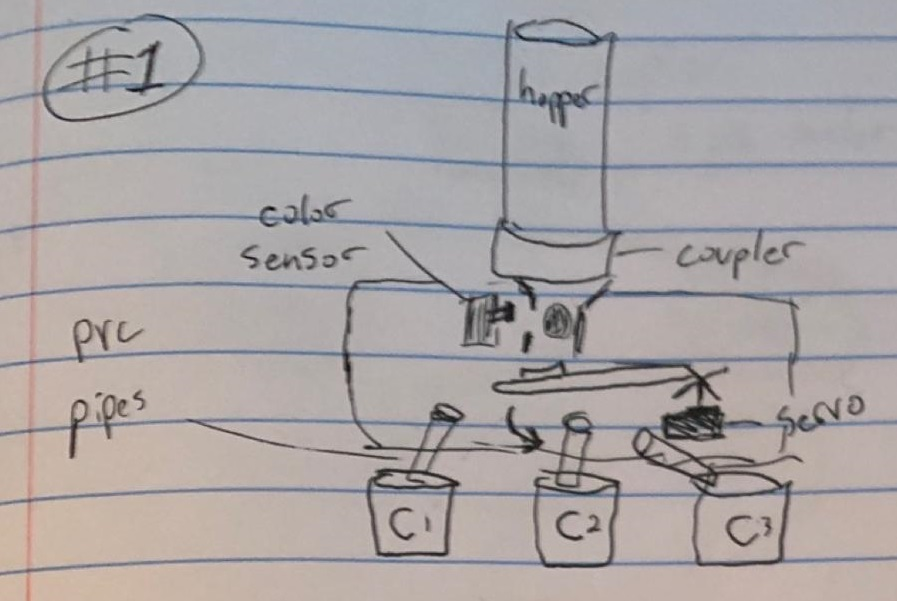
\includegraphics[width=\textwidth]{cg_1.jpg}\\
    \small{\textbf{Figure 4.5.1} - Tri-Tube}\\~\\
    
    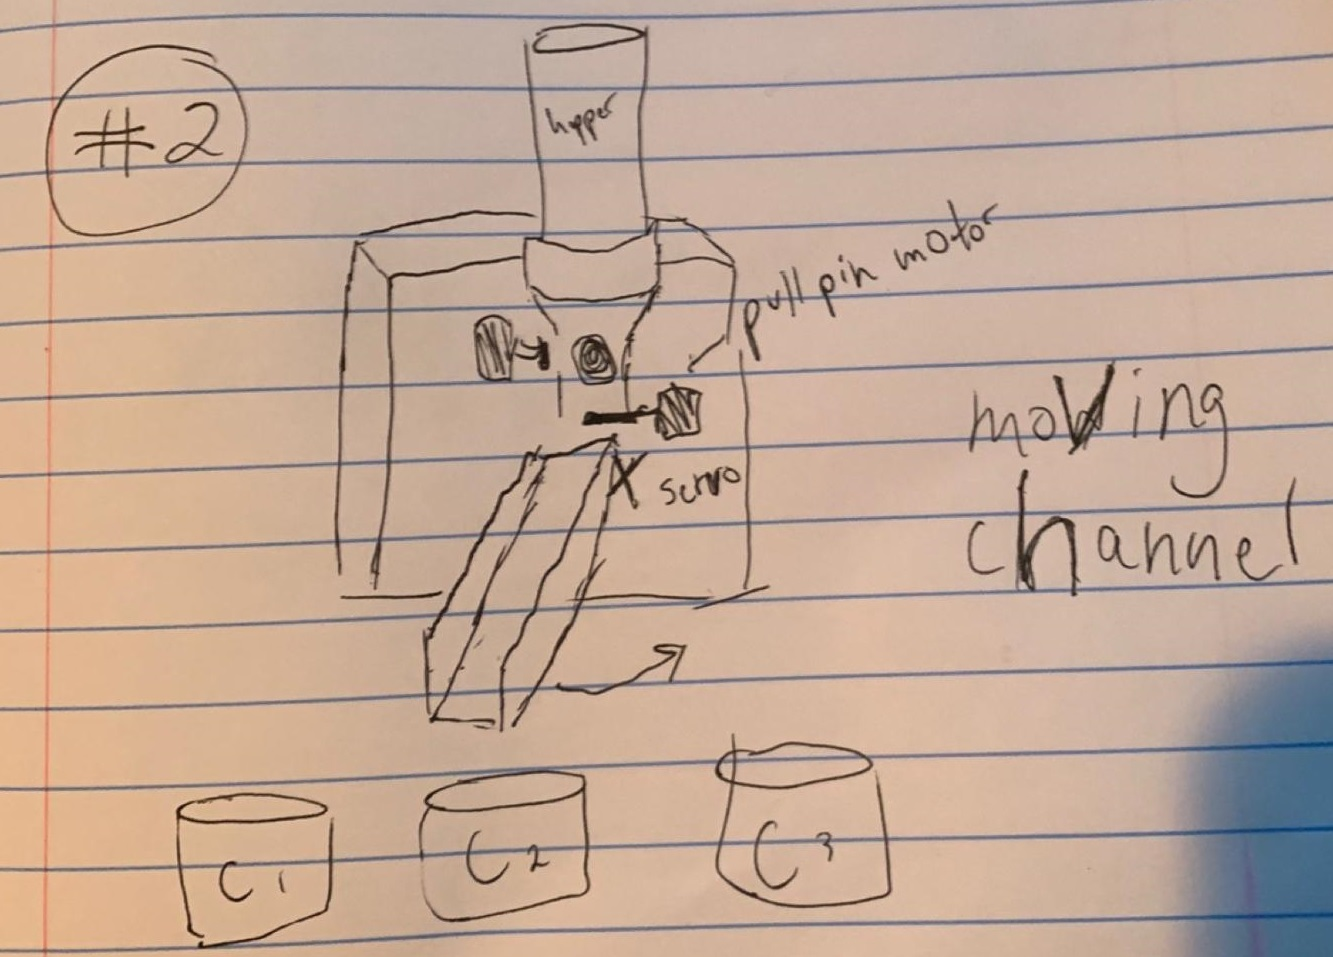
\includegraphics[width=\textwidth*0.9]{cg_2.jpg}\\
    \small{\textbf{Figure 4.5.2} - Moving Channel}\\~\\
    
    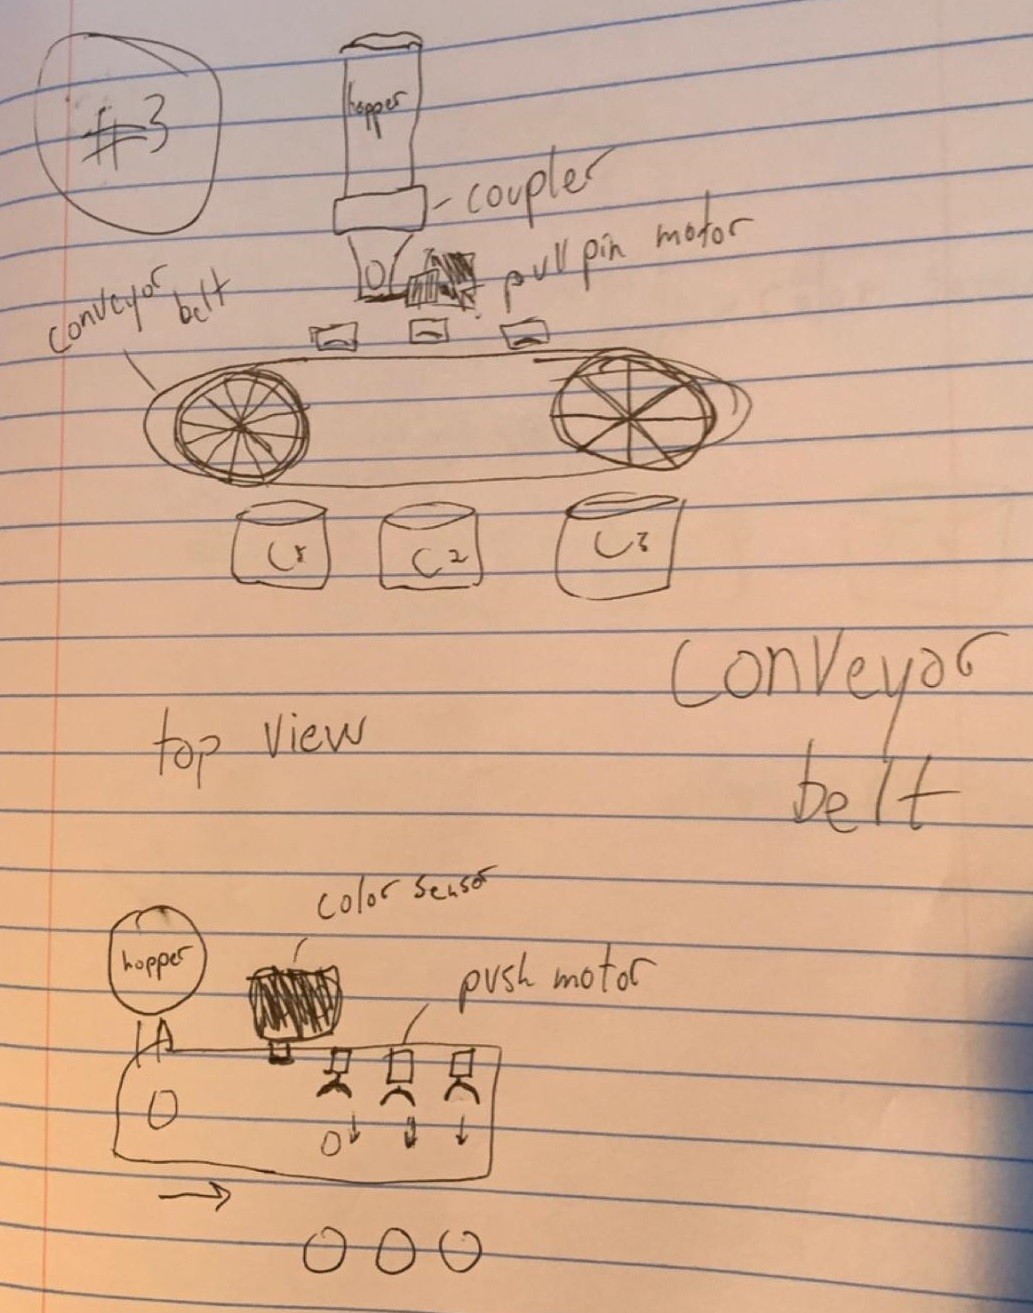
\includegraphics[width=\textwidth]{cg_3.jpg}\\
    \small{\textbf{Figure 4.5.3} - Conveyor Belt}\\~\\
    
    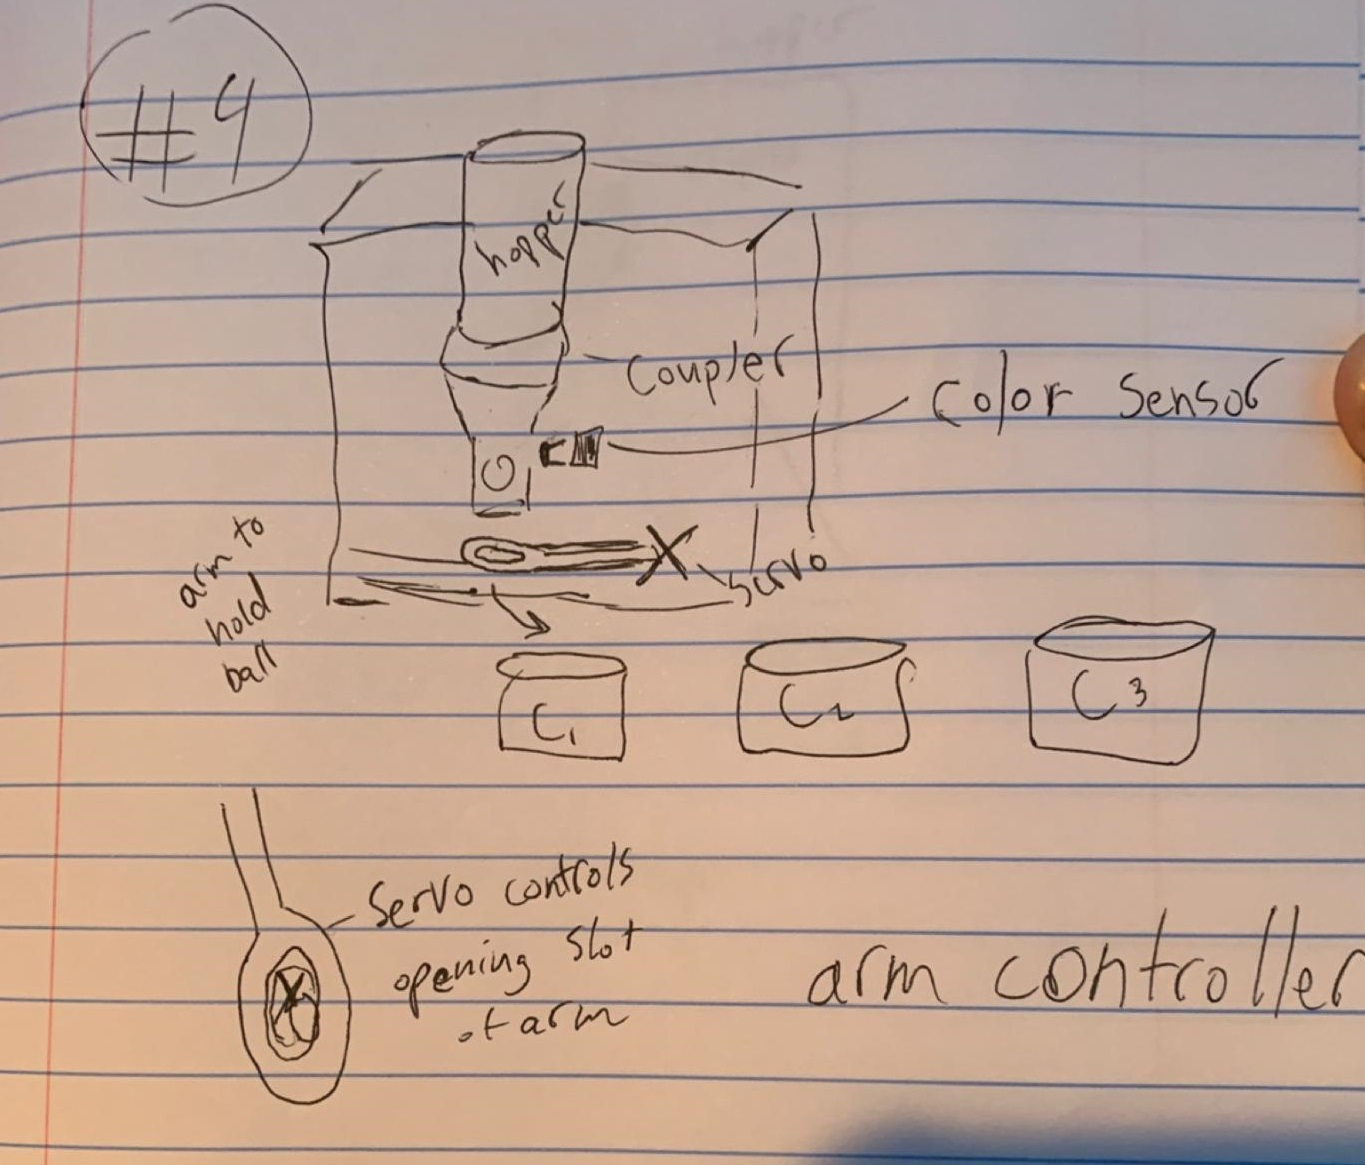
\includegraphics[width=\textwidth]{cg_4.jpg}\\
    \small{\textbf{Figure 4.5.4} - Arm Controller}\\~\\
    
    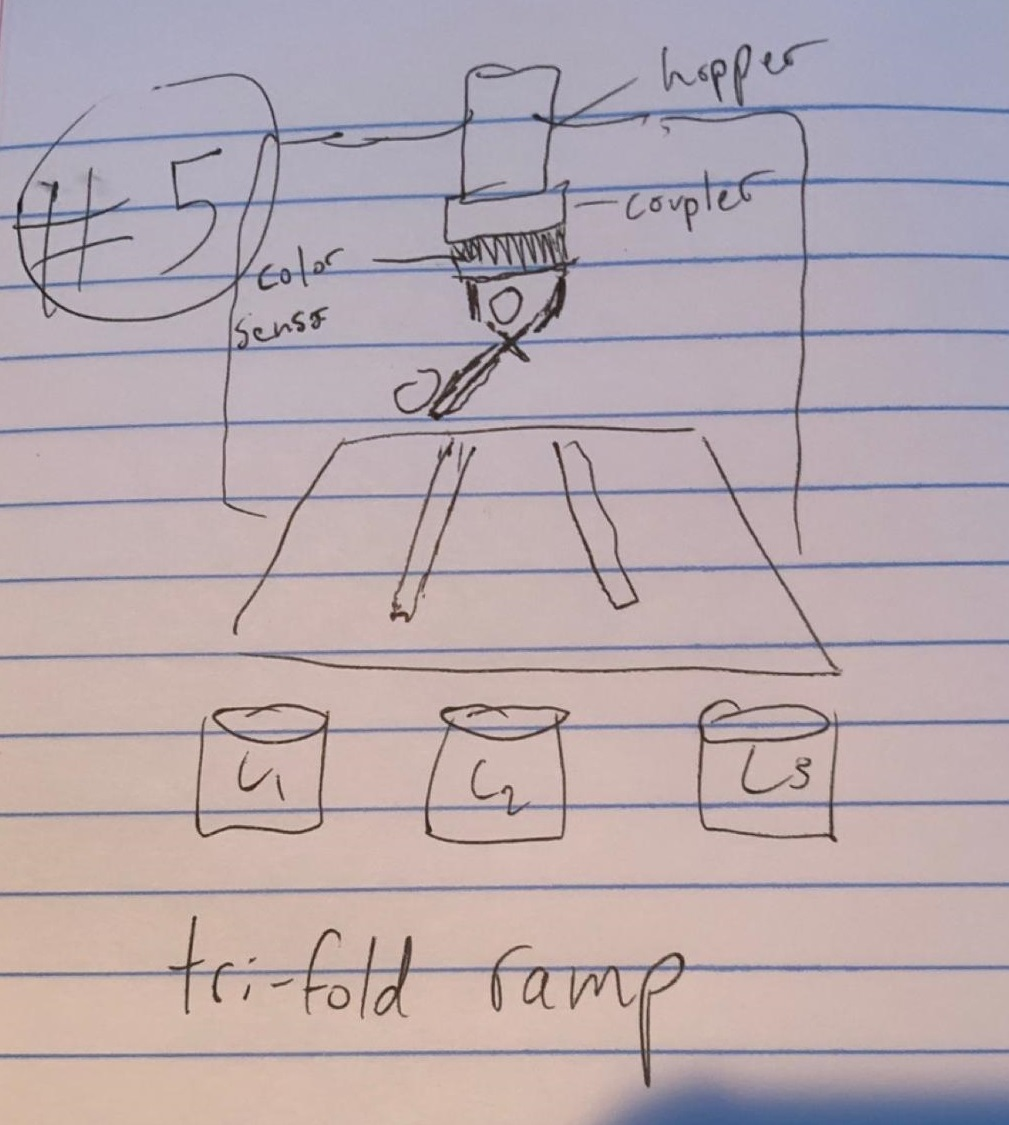
\includegraphics[width=\textwidth]{cg_5.jpg}\\
    \small{\textbf{Figure 4.5.5} - Tri-fold Ramp}\\~\\
    
\end{center}

\subsection{Comparison Chart}

\begin{center}
        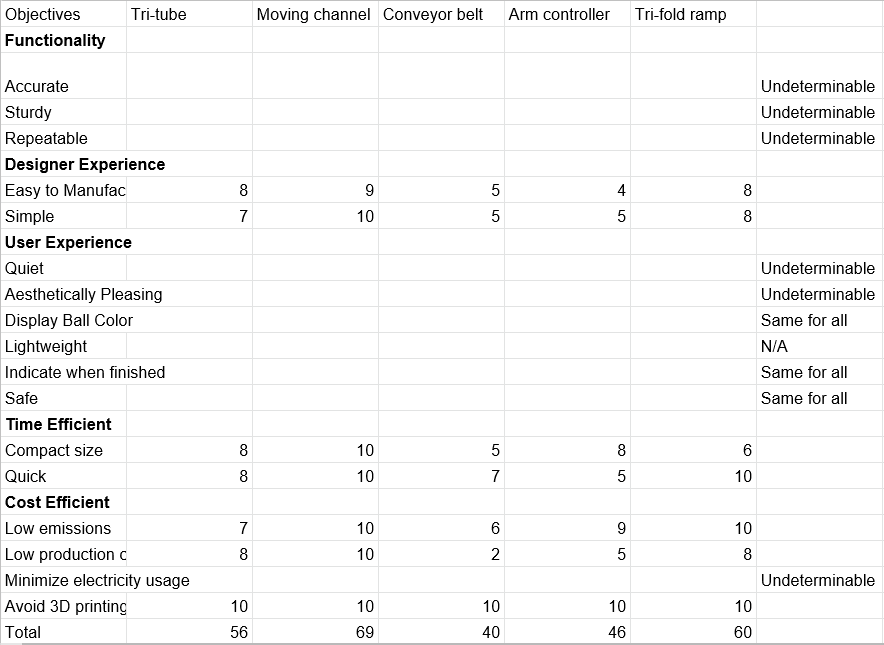
\includegraphics[width=\textwidth]{comparisonchart.png}\\
    \small{\textbf{Table 4.6.1} - Comparison Chart}\\~\\
\end{center}

The above chart, Table 4.6.1, was used to compare the top five concepts to select the top three designs and the best design. Each objective that could be determined from the initial designs was ranked from 1-10 with 10 being the highest. The scores were then summed, with the top design being the one one the highest sum. \\
Many of the objectives were given a rating of "Undeterminable" if it was not possible to determine from the initial design. Notably, there was some difficulty in finding the appropriate way to predict many of the secondary objectives in the functionality objective. Other objectives were given a rating of "Same for All" or "N/A" if it was determined that all designs would perform roughly the same for that objective.

\subsection{Conclusions}

In accordance with the purpose of this section, the most important parts of this section are the morphological chart, the comparison chart and the concepts lists and explanations for reductions in means. The morphological chart is of great importance as it is what is primarily used in order to generate all the different types of concepts. The explanations of the process taken to reduce the number of possible concepts is of great importance as it is how we come to closer to a limited amount of concepts. The comparison chart is of great importance as well as it presents the rankings that we performed in evaluating the best concept. Using the comparison chart we ultimately arrived as the moving channel concept as being the best as it ranked best in cost and time efficiency and was also the top performer in the objective of designer experience. This design was chosen to be our final design and will be detailed more thoroughly in the `Final Design' section.


\newpage
\section{Final Design}
\subsection{Introduction}
This section documents how the design was created from the original concept. The first subsection is the mechanical design, which details how we came up with the physical construction of the device, how we designed it with CAD, and how we created it; it includes CAD drawings of the design at different stages of development and explanations and rationale for why those changes were made. The second subsection is the electrical design, which contains detailed explanations of both how the hardware was configured and how the software was designed; to illustrate the electrical design, both a photograph and wiring diagram of the circuit are provided. Finally, the third subsection is the cost, which breaks down how expensive the device was to produce, based on both a bill of materials with dollar value and an environmental impact report that finds the footprint of each individual component.
\subsection{Mechanical Design}
\subsubsection{Preliminary Design}

\begin{center}
    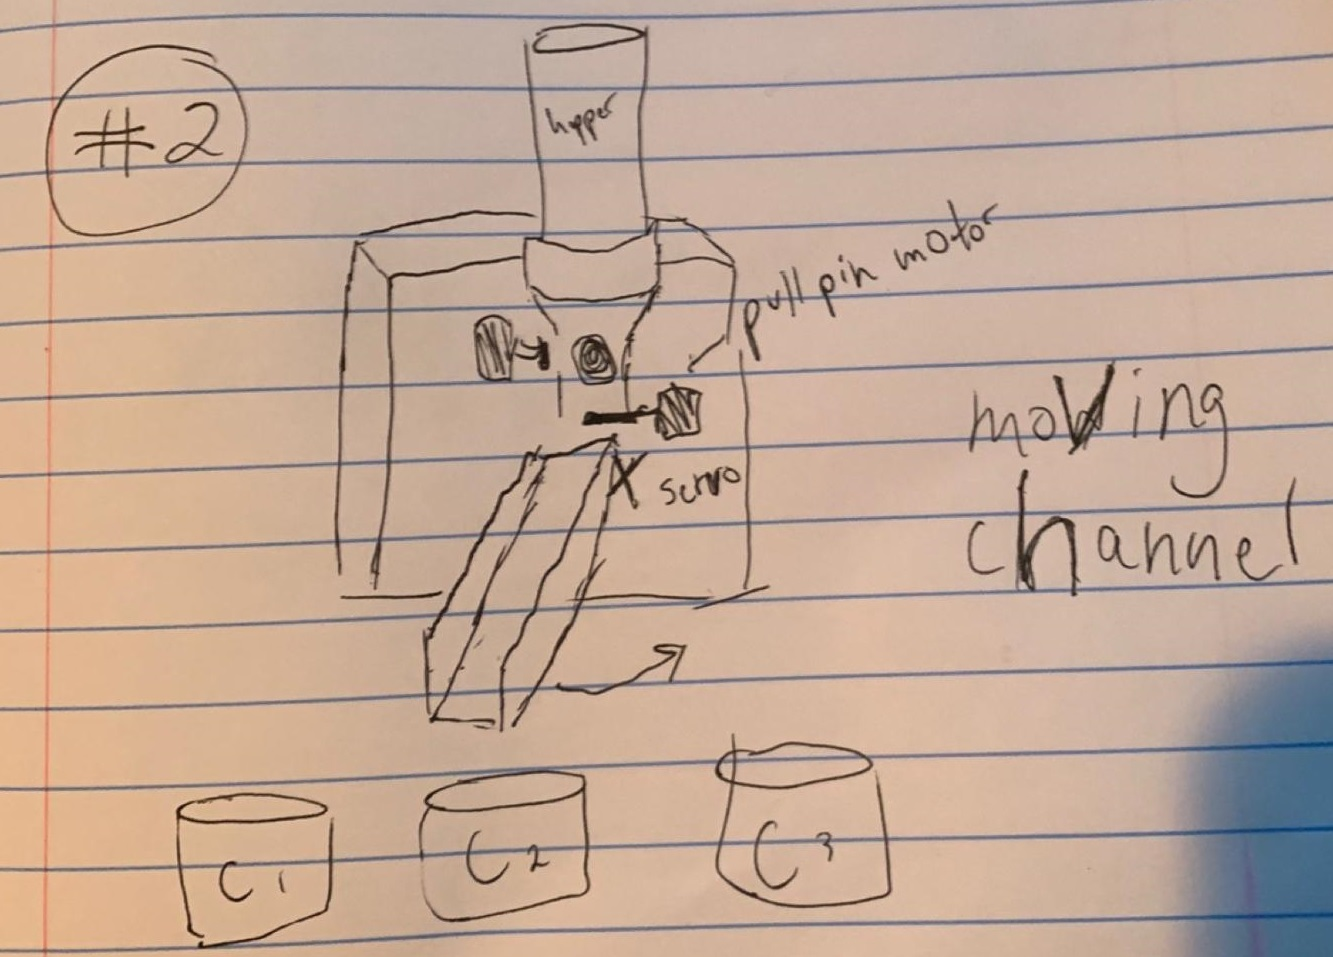
\includegraphics[width=\textwidth]{cg_2.jpg}\\
    \small{\textbf{Figure 5.2.1.1} - Moving Channel}\\~\\
\end{center}

\subsubsection{Prototype}

This design was the first attempt at recreating the idea from the drawing in CAD. The device is made mainly using 1/8" plywood, except for the stepper horn which is 3D printed. The top plate of the device has a large hole which can hold the outside diameter of the hopper, followed by a plate with a small hole that does not let the hopper tube pass through but lets the balls through. Below that, a stepper motor rotates a plate with 3 holes. This middle plate is close enough to the hole that a ball cannot drop down from the upper plate unless the hole in the wheel is aligned with the hole in the upper plate. The wheel then rotates the ball along the middle plate until is next to the color sensor, which detects the color of the ball and sends it to the Arduino. Next, a servo motor attached to the ramp via a ramp bracket rotates so that the ramp points towards the correct bin. The wheel rotates again, which simultaneously loads in another ball, rotates the previously loaded ball to the scanner, and rotates the just-scanned ball to a hole in the middle plate where it will fall onto the ramp and roll into the correct bin. The lower plate has a hole cut to house the servo, as well as a small round cut in the side of it so that the ramp has a wider range of mobility before it hits the plate. The pieces were mostly to be glued together to avoid the need for lots of fasteners such as screws and bolts. Overall the prototype design was a first draft at realizing the initial drawing and helped us conceptualize how our design would work before we built it.

\begin{center}
    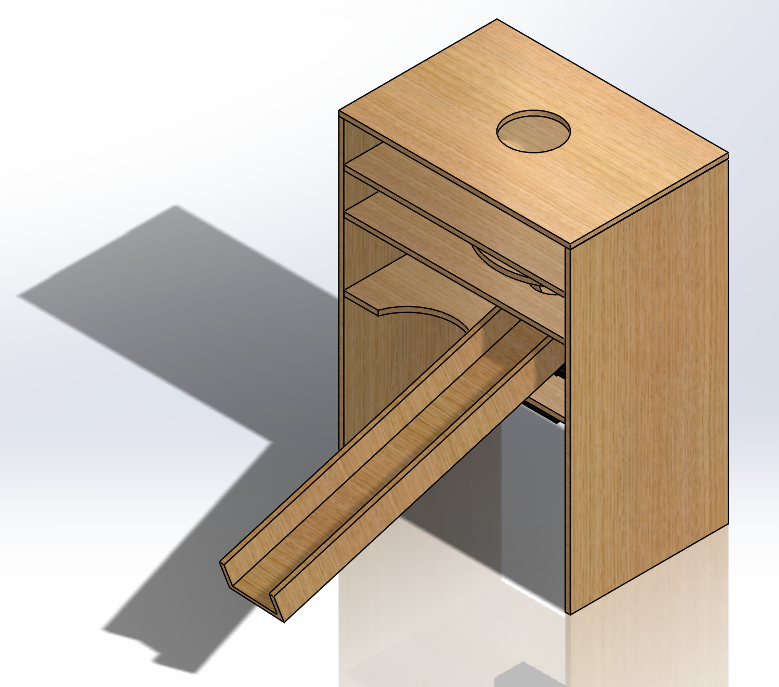
\includegraphics[width=\textwidth]{assembly_OLD.png}\\
    \small{\textbf{Figure 5.2.2.1} - Prototype CAD Assembly}\\~\\
\end{center}

\subsubsection{``In Progress" Redesign}

This design was created after the initial design when the group moved from the designing phase to the building phase. The most notable change was that all the wood pieces are now made of 1/4" wood instead of 1/8" like the original design, and the wheel is made of 1/8" laser-cut acrylic instead of hand-machined plywood. The wood was changed to 1/4" plywood both because the group determined 1/8" may not be sturdy enough, and because the lab did not have a large enough supply of 1/8". The wheel was switched to laser-cut acrylic since the group determined it would be too time consuming to accurately cut a circular wheel by hand. Overall, the design remained mostly the same, with only some changes made to better reflect the work environment that the group had access to.

\begin{center}
    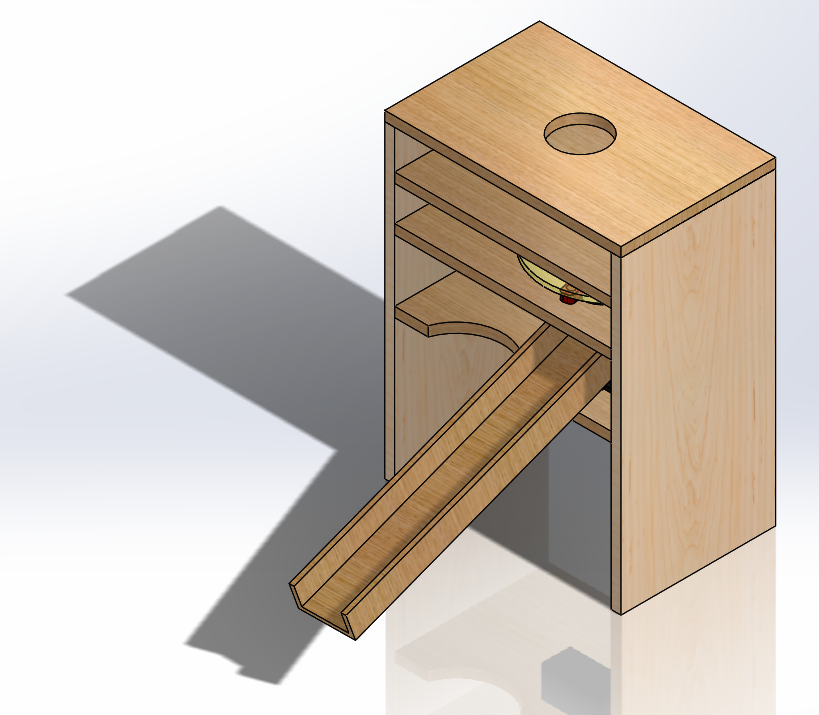
\includegraphics[width=\textwidth]{assembly_IP.png}\\
    \small{\textbf{Figure 5.2.3.1} - ``In Progress" CAD Assembly}\\~\\
\end{center}

\subsubsection{``As Built" Design}

The ``As Built'' design is notably different from the previous iterations. The most drastic change is that the pieces are now attached using screws instead of glue, which required some mild redesigning. The materials used were primarily OSB and MDF, which both would not hold well if a screw was drilled into the side. To fix this problem, supports were created out of 2x4s, which then had holes drilled into them to attach the pieces together at right angles. To space the section with the wheel properly, the upper plate was moved to be flat against the same support beams used for the top plate. Other small changes included the ramp material changing from plywood to cardboard since it was easier to create and weighed less, causing less strain on the servo. The color sensor was also relocated from the side wall to above the wheel so that it could get a more accurate reading as well as being more easily mounted and managed. The hole in the upper plate was widened to make room for a PVC coupler that could hold the hopper, as well as featuring a diversion ramp that ensured the ball was in the correct spot.

Dimensioned CAD drawings are available for this part below since it was the final iteration. For detailed drawings of the other components, see Appendix C.

\begin{center}
    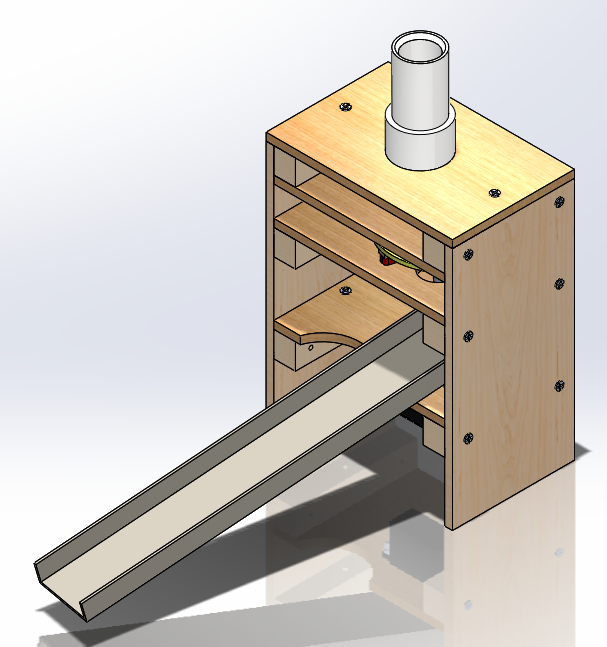
\includegraphics[width=\textwidth]{assembly_AB.png}\\
    \small{\textbf{Figure 5.2.4.1} - ``As Built" CAD Assembly}\\~\\
\end{center}

\subsection{Electrical Design}
\subsubsection{Hardware}

    The following session will describe the hardware used for the project. The table 5.3.1.1 shows the quantity of hardware and the description of each hardware and figure 5.3.1.2 shows a circuit diagram of the hardware.
    
    \begin{center}
    \begin{tabular}{|c|c|c|c|}
    \hline
       \textbf{\#}  & \textbf{Name} & \textbf{Qty} & \textbf{Description}  \\
       \hline
        1 & Arduino & 1 & Controls the device\\
        2 & Small breadboard & 2 & Connect hardware\\
        3 &  RGB LED & 1 & Shows signals from Arduino\\
        4 & Stepper Motor & 1 & Rotates wheel \\
        5 & Servo Motor & 1 & Rotates ramp \\
        6 & Resistor & 1 & 10k$\Omega$, protects LED from blowing out\\ 
        7 & Color Sensor & 1& Reads color value \\
        8 & Power Supply & 1 & Supplies power to motors\\
        \hline
    \end{tabular}
    
    \small{\textbf{Table 5.3.1.1} - Circuit Materials}\\~\\
    
    \end{center}

\subsubsection{Software}

\subsection{Cost}
\subsubsection{Bill of Materials}
\subsubsection{Environmental Impact}

\newpage
\section{Device Testing}

\newpage
\section{Conclusions}

\newpage
\appendix
\section*{Appendices}
\section{References}

\begin{enumerate}[start=1,label={[\bfseries \arabic*]}]
    \item C. L. Dym, P. Little, and E. Orwin, “Engineering Design: A Project Based Introduction 4th Edition,” pp. 92.
\end{enumerate}

\section{Code}
\subsection{Screenshots of Code}

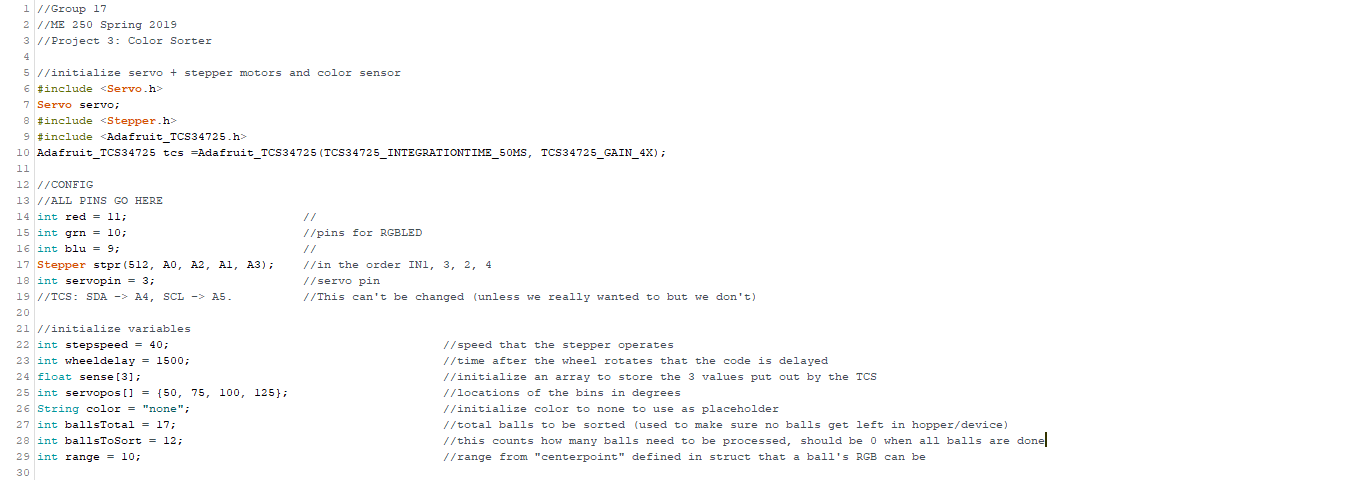
\includegraphics[width=\textwidth]{Screenshot_96.png}\\
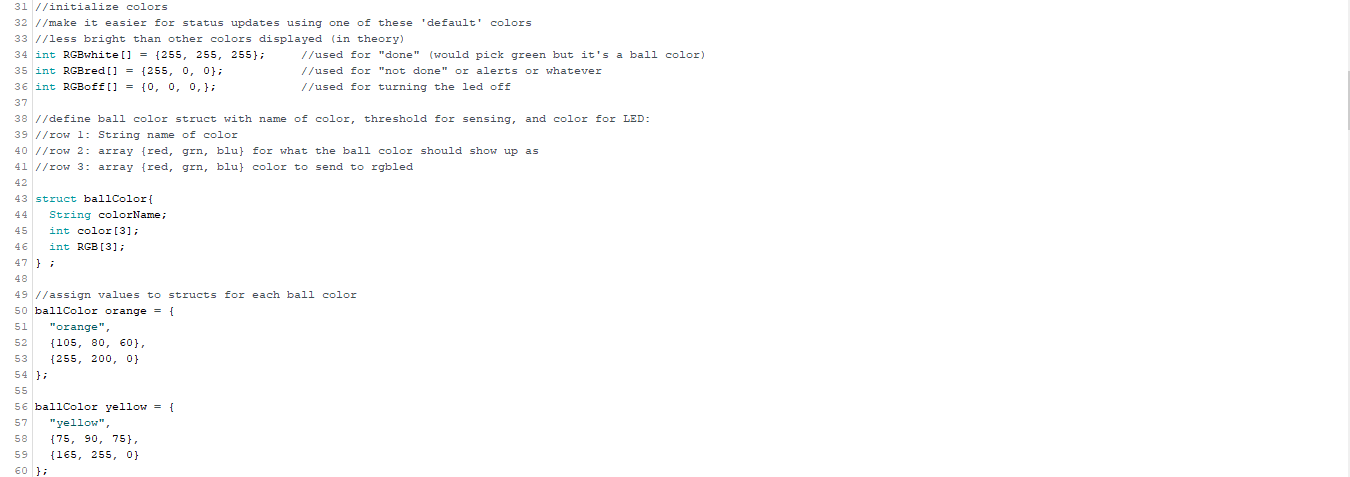
\includegraphics[width=\textwidth]{Screenshot_97.png}\\
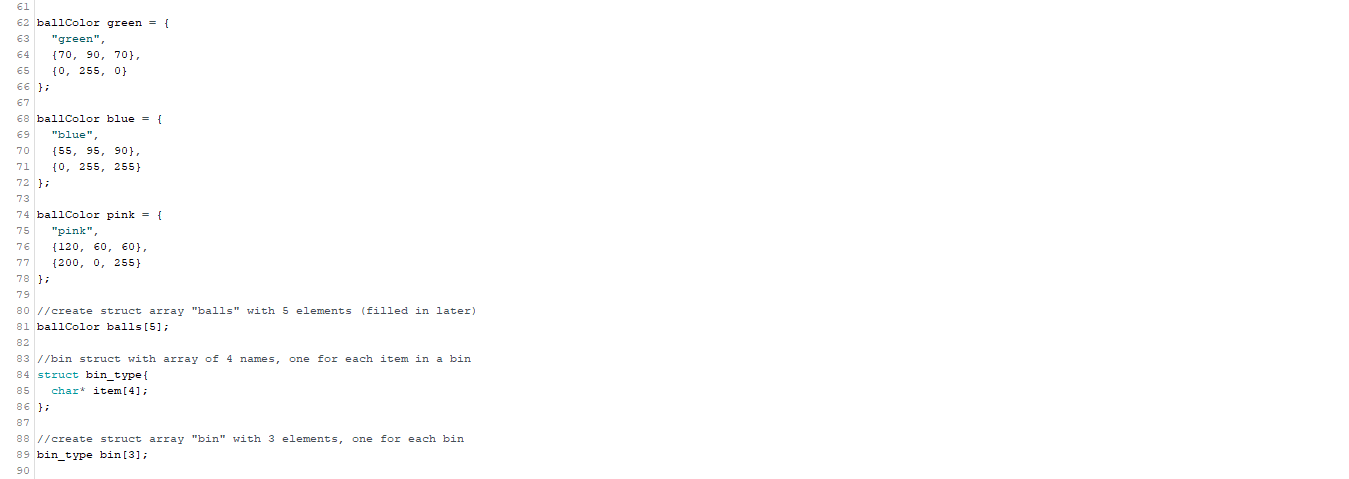
\includegraphics[width=\textwidth]{Screenshot_98.png}\\
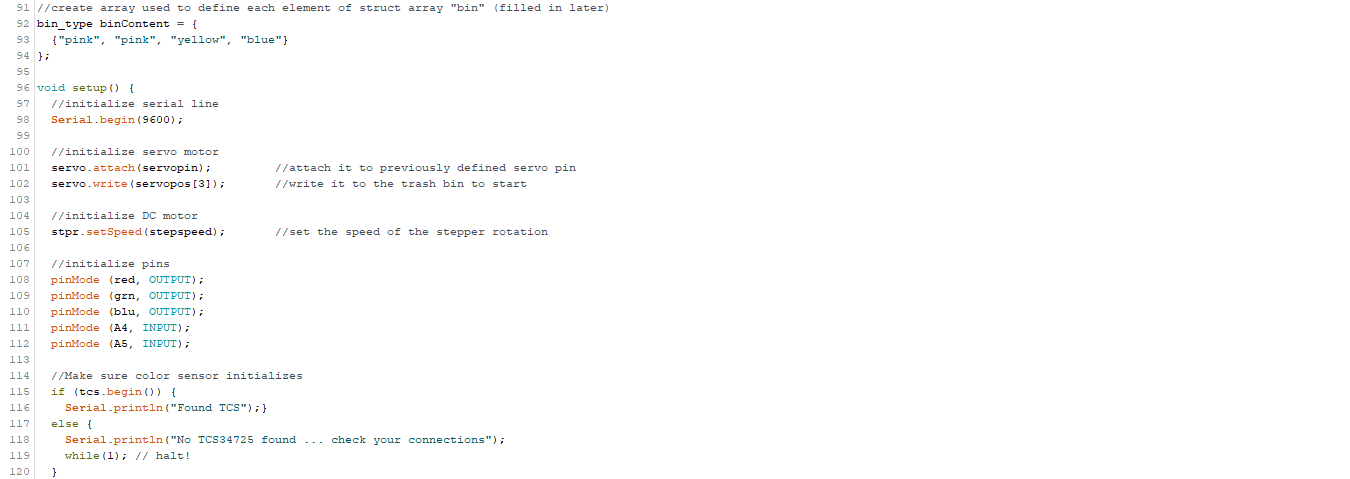
\includegraphics[width=\textwidth]{Screenshot_99.png}\\
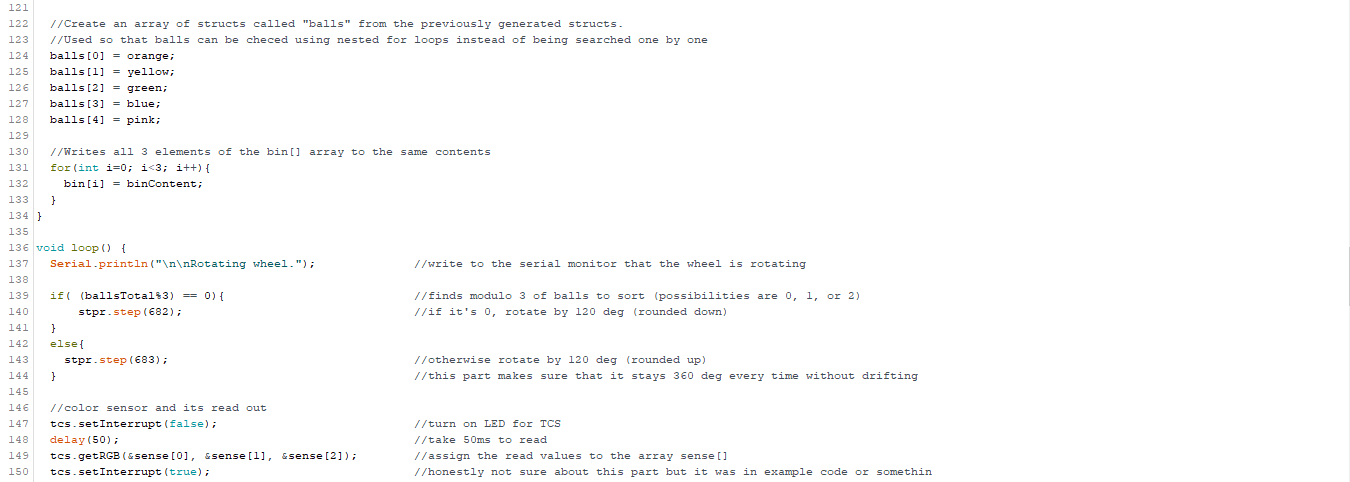
\includegraphics[width=\textwidth]{Screenshot_100.png}\\
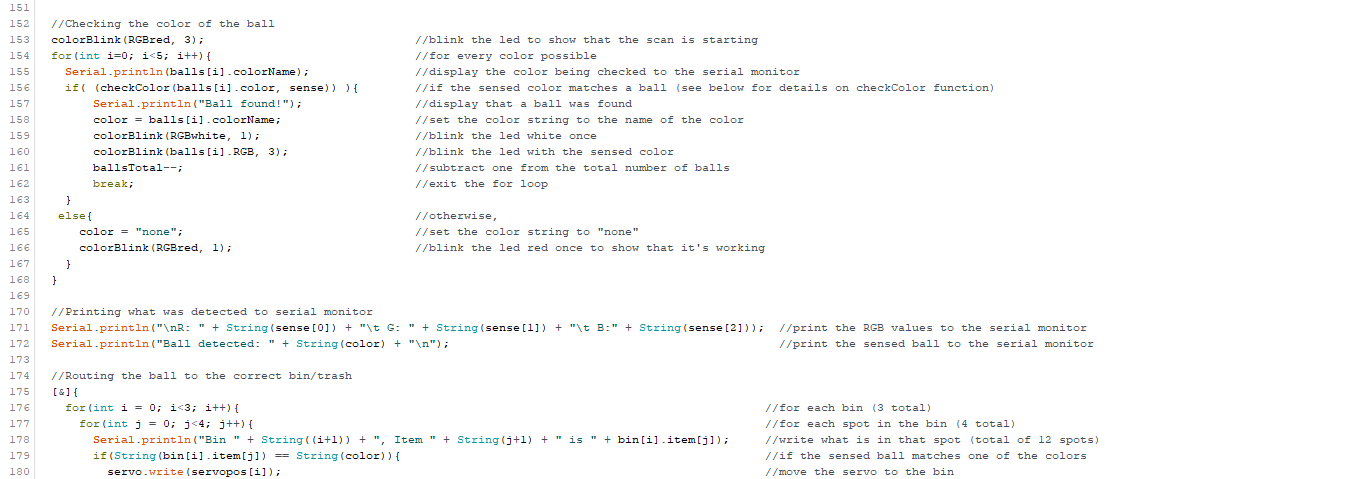
\includegraphics[width=\textwidth]{Screenshot_101.png}\\
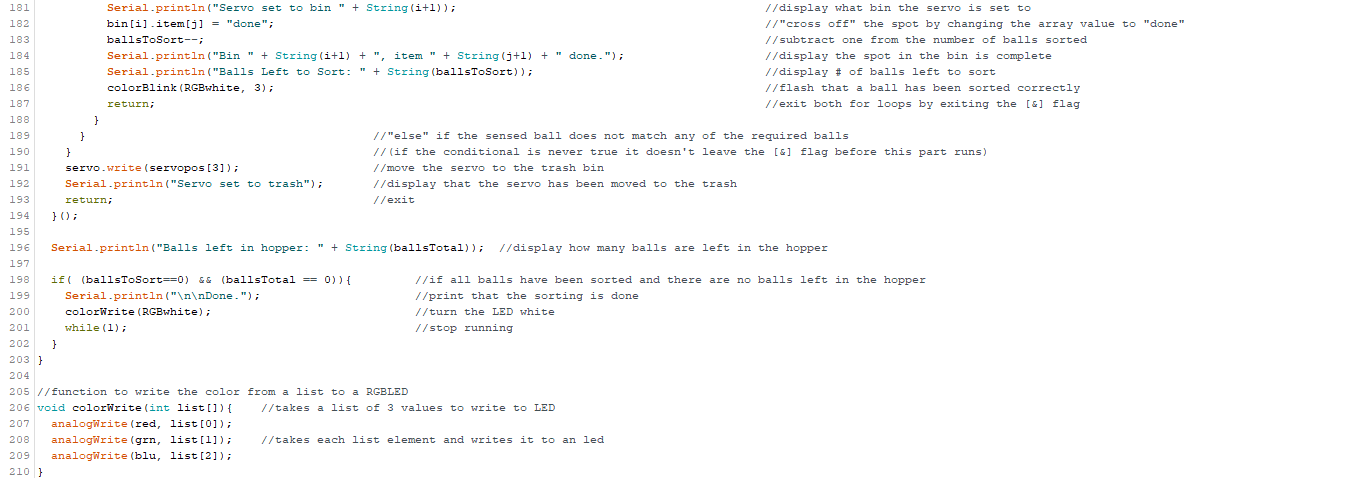
\includegraphics[width=\textwidth]{Screenshot_102.png}\\
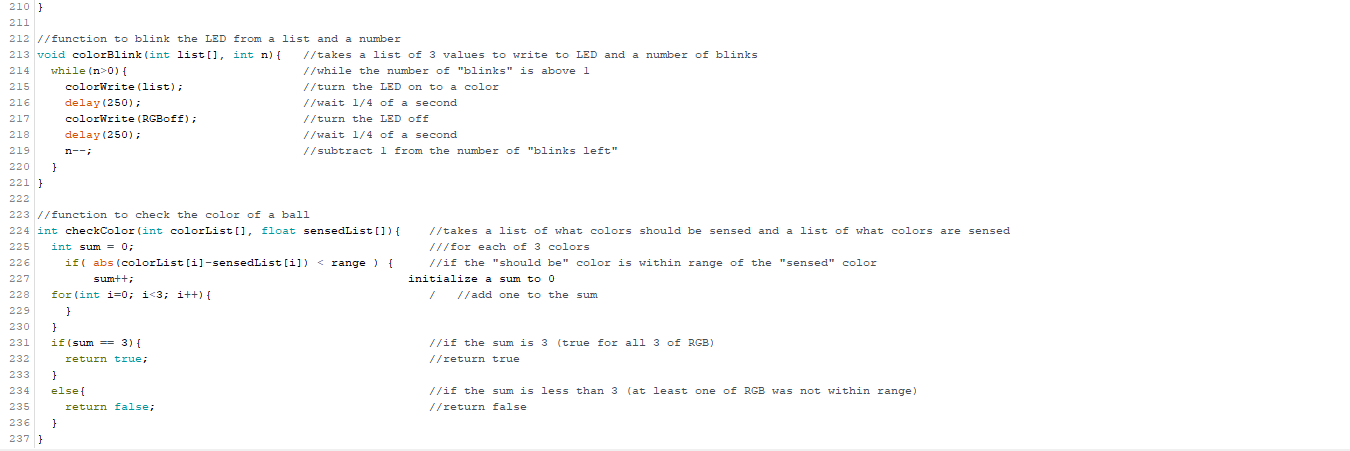
\includegraphics[width=\textwidth]{Screenshot_103.png}\\

\subsection{GitHub}
    Code for this project was maintained in a GitHub repository by Hammad Imam. The main Arduino code used in this project can be seen in more detail \href{https://github.com/himam99/ME250-Proj3/blob/master/Code/me250_proj3_code/me250_proj3_code.ino}{here.} Other code used in the development and testing of this project can be found \href{https://github.com/himam99/ME250-Proj3/tree/master/Code}{here.} Any questions about the GitHub repository can be sent to himam4@uic.edu.
    
\section{CAD}
\subsection{About}

All CAD work for this project was done in SolidWorks.

\subsection{Additional Files}

All drawings for the ``As Built" design are given above. The original part and assembly files, as well as the files for previous iterations of the design, can be seen \href{https://github.com/himam99/ME250-Proj3/tree/master/CAD}{here.}

\end{document}
